%  PHDTHESIS TEMPLATE FILE
%  Adopted from Thomas Fabricius and Henrik Aalborg Nielsen
%  Jan Larsen, IMM, DTU, Nov 2003 ver 1.0
%  Updated by Finn Kuno Christensen, fkc@imm.dtu.dk Aug 15, 2008

%  COMPILATION STEPS USING INVOLVING A PS FILE
%\documentclass[10pt,twoside,dvips]{book}
%  latex phdthesis.tex
%  dvips -D600 -Pamz -Pcmz -j0 phdthesis.dvi -o phdthesis.ps
%  ps2pdf -sPAPERSIZE#b5 phdthesis.ps phdthesis.pdf (or use Acrobat Distiller)

%  COMPILATION STEP USING PDFLATEX
\documentclass[10pt,twoside]{book}
%  pdflatex thesis.tex

%%%%%%%%%%% MODIFY THESE LINES ONLY %%%%%%%%%%%%%%%%%%%%%%%%%%%%%%%%%%%%%%%%%%%%%%%%%%%%%%%%%
\def\thesisyear{2012} % Year thesis submitted
\def\thesisnumber{??}  % Only number no year
\def\thesisauthor{Michael Lun�e} % Thesis author
\def\thesistitle{Personalising the Editorial Mix for a Digital Newspaper using Constraint Programming} % Title of thesis
\def\thesiskeywords{constraint programming, editorial mix, personalisation}
\def\thesisISBN{????-????} %OBSOBS provide ISBN number for industrial phd students ONLY
\def\thesisversion{print} %OBSOBS choose this for printed version send to printing
%\def\thesisversion{net} %OBSOBS choose this for the net version for the web and publication database
%%%%%%%%%%%%%%%%%%%%%%%%%%%%%%%%%%%%%%%%%%%%%%%%%%%%%%%%%%%%%%%%%%%%%%%%%%%%%%%%%%%%%%%%%%%%%

\newcommand{\np}{$\mathcal{NP}$}

%!TEX root = thesis.tex
\usepackage[utf8]{inputenc}
\usepackage[english]{babel}
\usepackage{ae} %danish ae, oe and aa
\usepackage{lib/fancyheadings}
\usepackage{amsmath,amssymb,latexsym,epic,eepic,graphicx,graphics}%epsfig,psfrag
\providecommand{\abs}[1]{\lvert#1\rvert}
\usepackage{theorem}
\usepackage{lib/immthesislayout}
\usepackage[justification=centering]{caption}

% figures
\usepackage{rotating}
\usepackage{subfigure}

% Bibliography
\usepackage{lib/named}
%\usepackage{lib/authordate1}
%\usepackage{lib/apacite}

% Defintion environment
\newtheorem{mydef}{Definition}

% Pseudocode
\usepackage{url}
\usepackage{verbatim}
\usepackage{fancyvrb}
\usepackage{lib/clrscode3e}
\usepackage{listings}

\usepackage{todonotes}
\newcommand\todonote[1]{\textcolor{red}{\todo[bordercolor=red,backgroundcolor=white,inline]{? #1}}}

% Sourcecode
%\usepackage[usenames,dvipsnames]{pstricks}
%\usepackage{courier}
%\usepackage{pst-node}
\usepackage{xcolor,xspace}
\usepackage{color}
\sloppy
\definecolor{DarkBlue}{rgb}{0,0.08,0.45}
\definecolor{DarkGreen}{rgb}{0,0.50,0.00}

\lstset{
extendedchars=\true,            %æ,ø,å
%language=ML,                    % choose the language of the code
basicstyle=\footnotesize\tt,    % the size of the fonts that are used for the code
numbers=left,                   % where to put the line-numbers
numberstyle=\footnotesize,      % the size of the fonts that are used for the line-numbers
stepnumber=2,                   % the step between two line-numbers. If it's 1 each line will be numbered
numbersep=5pt,                  % how far the line-numbers are from the code
backgroundcolor=\color{white},  % choose the background color. You must add \usepackage{color}
showspaces=false,               % show spaces adding particular underscores
showstringspaces=false,         % underline spaces within strings
showtabs=false,                 % show tabs within strings adding particular underscores
frame=single,	                % adds a frame around the code
tabsize=1,	                    % sets default tabsize to 2 spaces
captionpos=b,                   % sets the caption-position to bottom
breaklines=true,                % sets automatic line breaking
breakatwhitespace=false,        % sets if automatic breaks should only happen at whitespace
commentstyle=\color{DarkGreen},
keywordstyle=\color{DarkBlue}\bfseries,  % color of kw's
title=\lstname,                 % show the filename of files included with \lstinputlisting; also try caption instead of title
}

\def\thesisISSN{????-????}
\def\ttitle{{\sf\textbf{\thesistitle}}}
\def\thesisdef{IMM-BSc-\thesisyear-\thesisnumber}
\usepackage[b5paper]{hyperref}
\def\printversion{print}
\ifx\thesisversion\printversion
  %\special{papersize=176mm,250mm}
  \hypersetup{pdftitle={\thesistitle},
              pdfauthor={\thesisauthor},
              pdfsubject={\thesisdef},
              pdfkeywords={\thesiskeywords},
              breaklinks,
              bookmarksopen,
              bookmarksnumbered}
\else
  \hypersetup{pdftitle={\thesistitle},
              pdfauthor={\thesisauthor},
              pdfsubject={\thesisdef},
              pdfkeywords={\thesiskeywords},
              colorlinks,
              linkcolor=blue,
              breaklinks,
              bookmarksopen,
              bookmarksnumbered}
\fi

\newcommand{\papertitle}{}
\setcounter{tocdepth}{1} % 1 in final version 10 for debugging
\setcounter{secnumdepth}{3} % subsubsections get a number when this is 3
\begin{document}

%!TEX root = thesis.tex
\thispagestyle{empty}
\vspace*{\fill}
\begin{center}
\hspace{-6.64mm}{\huge\sffamily\bfseries Personalising the Editorial Mix}\\*[2.5cm]
\vspace{-24.5mm}\hspace{-6.64mm}{\huge\sffamily\bfseries for a Digital Newspaper}\\*[2.5cm]
\vspace{-24.5mm}\hspace{-6.64mm}{\huge\sffamily\bfseries using Constraint Programming}\\*[2.5cm]
\vspace{24.5mm}\hspace{-6.64mm}\Large\sf\thesisauthor\\*[4.5cm]
\hspace{-6.64mm}\small\sf Kongens Lyngby \thesisyear\\
\small\sf\hspace{-6.64mm} IMM-MSc-\thesisyear-\thesisnumber


\end{center}
\vspace*{\fill}
\newpage
\thispagestyle{empty}
\vspace*{11cm}
{\sf Technical University of Denmark}\\
{\sf Informatics and Mathematical Modelling}\\
{\sf Building 321, DK-2800 Kongens Lyngby, Denmark}\\
{\sf Phone +45 45253351, Fax +45 45882673}\\
{\sf reception@imm.dtu.dk}\\
{\sf www.imm.dtu.dk}

\vspace*{2.5cm}
\def\empty{}
\ifx\thesisISBN\empty
 {\sf IMM-MSc: ISSN \thesisISSN}
\else
  {\sf IMM-MSc: ISSN \thesisISSN, ISBN \thesisISBN}
\fi

% PREFACE CHAPTERS INCLUDE
\frontmatter
\pagenumbering{roman}

%!TEX root = thesis.tex
\chapter{Abstract}

%The thesis establishes the theory of Constraint Programming (CP) and playlists. It applies techniques of CP, logic and functional programming with a similarity function between music pieces to build an Automatic Playlist Generator. The product of the thesis is a program in SML that generates playlists from a users query of suggestions and bans of songs. The similarity function is build solely on measures in tempo and key, which results in playlists that are somewhat useless. The program lack of measures in timbre, rhythm and melody, but is left open for the implementation of these. The thesis finally concludes that the techniques of CP and local search proves efficient for solving the problem.

\markboth{}{}
%!TEX root = thesis.tex
%\chapter{} %{Sammenfatning (Summary in Danish)}

\pdfbookmark[1]{Resum\'e}{Resum\'e} % Bookmark name visible in a PDF viewer

\begingroup
\let\clearpage\relax
\let\cleardoublepage\relax
\let\cleardoublepage\relax

\chapter*{Resum\'e} % Abstract name

Kort resum\'e af indholdet\dots
%Projektet præsenterer den grundlæggende teori bag Constraint Programming (CP) og playlists. Strategien i arbejdet med constraints, logisk og funktionel programmering er anvendt til at opstille en Automatic Playlist Generator, som også benytter sig af en funktion til at sammenligne musiknumre. Produktet af projektet er et program i SML der genererer playlists ud fra forslag og forbud på sange fra et bibliotek. Funktionen til sammenligning er alene baseret på sammenligning imellem tempo og toner (key), som resulterer i forholdsvist ubruglige playlists. Programmet mangler sammenligninger imellem klangfarve (timbre), rytme og melodi, men den dynamiske tilgang gør at det let kan implementeres. Til sidst sluttes af den anvendte CP og local search tilgang viser sig effektiv til at løse problemet.

\endgroup			

\vfill
\markboth{}{}
%!TEX root = ../thesis.tex
%\chapter{} %{Sammenfatning (Summary in Danish)}

\pdfbookmark[1]{Preface}{Preface} % Bookmark name visible in a PDF viewer

\begingroup
\let\clearpage\relax
\let\cleardoublepage\relax
\let\cleardoublepage\relax

\chapter*{Preface}
%Time spent on assembling playlists for certain purposes often exceeds the actual use. Some automatic playlist generation engines already exists, but they often lack the possibility of altering the generated playlist - or the option of specifying the length. The result is a repeated query for a playlist until one satisfies and another when it runs out of songs to play.
%
%This thesis is the product of a personal need for an Automatic Playlist Generator.
%
%The thesis is produced under the Department of Informatics and Mathematical Modelling at the Technical University of Denmark and it will presume some knowledge of logic programming and functional programming as it will include an implementation of a program in each language. The preconditions for the thesis are the courses 02156 Formal Logical Systems and 02157 Functional programming taught at the Technical University of Denmark.

\vspace{20mm}
\mbox{}\hfill
\begin{minipage}[t]{80mm}
  Kgs. Lyngby, \myDate
  \\ \\
  \mbox{} \hspace{-16mm} 
\includegraphics{img/signature.eps}
  \myName
\end{minipage}

\endgroup			

\vfill

\markboth{}{}
%\input{papers.tex} TODO:
%\markboth{}{}
%!TEX root = ../thesis.tex
% Acknowledgements

\pdfbookmark[1]{Acknowledgements}{Acknowledgements} % Bookmark name visible in a PDF viewer

\begin{flushright}{\slshape    
We have seen that computer programming is an art, \\ 
because it applies accumulated knowledge to the world, \\ 
because it requires skill and ingenuity, and especially \\
because it produces objects of beauty.} \\ \medskip
--- \defcitealias{knuth:1974}{Donald E. Knuth}\citetalias{knuth:1974} \citep{knuth:1974}
\end{flushright}

\bigskip

%----------------------------------------------------------------------------------------

\begingroup

\let\clearpage\relax
\let\cleardoublepage\relax
\let\cleardoublepage\relax

\chapter*{Acknowledgements} % Acknowledgements section text

\noindent I would like to thank my family and friends for support and review of the thesis. I would also like to thank my counsellors, Michael Kai Petersen and Carsten Witt from the Department of Informatics and Mathematical Modelling at the Technical University of Denmark, for giving me room for my own definition of the thesis. Also for review of the process and guidance in the right direction.

\endgroup

\markboth{}{}

% TABLE OF CONTENTS
\newpage\mbox{}\newpage
\chaptermark{Contents}
\renewcommand{\sectionmark}[1]{\markright{#1}}
\sectionmark{Contents}
\addtolength{\parskip}{-\baselineskip}
\tableofcontents
\addtolength{\parskip}{\baselineskip}
\renewcommand{\sectionmark}[1]{\markright{\thesection\ #1}}

% MAIN CHAPTERS INCLUDE
\mainmatter
%!TEX root = thesis.tex
\chapter{Introduction} % (fold)
\label{ch:introduction}

%\todonote{? Første side er vigtig for karaktergivningen. ``Det er komplekst det her, Nå, der er et bud på det... osv.''}
\section{Problem description}
% Optimising the Editorial Mix for a Digital Newspaper using Constraint Programming
% Optimering af den Redaktionelle Sammensætning i en Digital Avis med brug af Constraint Programmering
% start 6/2
% aflevering 3/8
% General project objectives:
% The overall objective of the project is to make the student familiar with Constraint Programming, especially Constraint Optimised Problems, and its uses in the context of personalisation. A specific personalisation problem is implemented and solved using Constraint Programming and relevant metaheuristics. Finally, the project provides a conceptual basis for developing personal digital solutions and the uses for Constraint Programming.
% Learning objectives:
% Explore existing literature and summarise it.
% Analyse the applicability of personalisation in a given domain and derive features of the problem to be personalised.
% Find applicable metaheuristics for personalisation problems and refine them accordingly.
% Model the identified features as constraints in a Constrained Optimisation Problem. Solve the defined Constraint Optimisation Problem in Constraint Programming.
% Evaluate Constraint Programming as a tool for personalisation problems and compare the solution to existing solutions.
% Describe and discuss the project in a report and present it orally.
%
%
% Revised Problem Specification:
\subsection{Title}
Personalising the Editorial Mix for a Digital Newspaper using Constraint Programming

\subsection{Danish Title}
Personalisering af den Redaktionelle Sammensætning i en Digital Avis med brug af Constraint Programmering

\subsection{Time Frame}
Project start 6/2-2012, delivery 3/8-2012.

\subsection{General Project Objectives}
The overall objective of the project is to make the student familiar with personalisation and the concept of modelling user preferences in digital solutions. A specific personalisation problem is analysed and relevant design proposals are discussed. A chosen design is implemented and solved using Constraint Programming. The project provides a conceptual basis for the use of Constraint Programming in the context of developing personalised digital solutions. Finally, the project attempts to make personalisation more accessible for developers with the introduction of Constraint Programming to the field.

\subsection{Learning Objectives}
Explore existing literature and summarise it.

Analyse the applicability of personalisation in a given domain and derive features of the problem to be personalised.

Identify features in the domain that can be solved using Constraint Programming.

Model the identified features as constraints and solve them using Constraint Programming.

Refine the identified features into general guidelines for the use of Constraint Programming in the context of personalisation.

Evaluate Constraint Programming as a tool for personalisation problems and compare the solution to existing solutions.

Describe and discuss the project in a report and present it orally.
% end of Revised problem spec

%\footnote{In constraint satisfaction, constrained optimization seeks for a solution maximizing or minimizing a cost function, Wikipedia.}
%\footnote{Personalization involves using technology to accommodate the differences between individuals, Wikipedia.}
The overall idea is to determine the use of Constraint Programming (CP) as a tool to make the personalisation of digital solutions more accessible.
\todonote{Footnote: definition of CP and definition of personalisation}

The project will be divided into two main areas; i.e.~an assessment of the use of CP in the context of personalisation and a direct application of this in the form of a personal digital news paper, where CP is used to personalise the content and composition of a digital newspaper.

\subsection{Personalisation Challenges}
In an attempt to personalise the content of a newspaper, the report will try to analyse which preferences the users will have with respect to the content and composition of relevant articles. It will describe the search for articles to fit the user needs as an Constraint Optimisation Problem and try to solve it. What makes a newspaper is not only the accumulated content of its articles, but the editorial mix of them. ``Which articles should go where'' is just as important and the composition of newspaper should therefore go through an equal solving process.
\todonote{Footnote: definition of COPs}

\subsection{Algorithmic Challenges}
To be able to use and assess CP in the context of personalisation a full understanding must be acquired. Features that can be solved using CP will be modelled as a COP and solved. Furthermore, because the problem has a fixed budget for finding a solution, its algorithmic complexity will be analysed. The findings will be concluded in an evaluation of the applicability of personalisation problems in CP.

\subsection{Existing solutions}
Personalisation of digital solutions becomes more common everyday and users demand personalised solution to accommodate their needs. Many solutions to this problem already exists, but the role of CP within this domain has not been determined. This project seeks to explore CP as a tool to make the personalisation of digital solutions more accessible.
%
%\subsection{Subproblem specification}
%Before evaluating the use of COPs with respect to personalisation it needs to be determined whether the problem can actually be described as a COP. Moreover, the editorial constraints needs to be defined. These will constitute a knowledge base of ground rules from which a paper will be generated. The article will look into current media,~i.e.\ radio programmes, television programmes, magazines and of cause news papers, to try to specify rules of layout and succession of articles based on metadata. The first part of this article will address this problem.
%
%A crucial part of the project is also to lay down the means of bringing content to the paper. A normal way to do this would be to use feeds or to scrape web sites (extracting information from web sites) of articles. The pros and cons of each method and further options needs to be addressed and an optimal solution chosen. This will constitute the second part of the article.
%
%
%
%
%bedste måde at inddrive den information vi skal bruge for at kunne arbejde med det og generere den digitale avis der passer dig bedst
%
%analyse - cop i dybden medier kan - synagien i et layout genskabes fra links og tweets?, design, implementation - web, anvende, test (evaluere). Realtion til playlist - som går på at få en stemning kommunikeret. Bygge en oplevelse - hver artikel bidrager til helheden. tværsnit. analyse=model+brugerpræferencer. topic (flere) vs. genre (én). grænseværdi for topics (hvor mange giver mening) granulalitet. genre i første omgang. analysere sig frem til sammensætning af ord => definere topics - distributioner af ord. mappe ord fra topic knowledge base til artikel. opbygge og glemme viden gradvist (1 måned eller 1 år?). Udvælge punkter der kunne være at undersøge.
%
%\subsection{General Project Objectives}
%The overall objective of the project is to make the student familiar with Constraint Programming, especially Constraint Optimised Problems, and its uses in the context of personalisation. A specific personalisation problem is implemented and solved using Constraint Programming and relevant metaheuristics. Finally, the project provides a conceptual basis for developing personal digital solutions and the uses for Constraint Programming.
%
%\subsection{Learning Objectives}
%Explore existing literature and summarise it.
%
%Analyse the applicability of personalisation in a given domain and derive features of the problem to be personalised.
%
%Find applicable metaheuristics for personalisation problems and refine them accordingly.
%
%Model the identified features as constraints in a Constrained Optimisation Problem.
%
%Solve the defined Constraint Optimisation Problem in Constraint Programming.
%
%Evaluate Constraint Programming as a tool for personalisation problems and compare the solution to existing solutions.
%
%Describe and discuss the project in a report and present it orally.

\section{Motivation}
The development of the Internet from a distributer of information to a library of digital applications has deeply integrated the users in every step of an applications lifetime. It has even become harder to distinguish between super users and developers, applications are branched and modified according to every need and authors can therefore no longer predict which use his or her application can be to another user - nor should he/she have to.

User preferences are very diverse and it is therefore hard to accommodate every individual in a single solution. A digital solution must be bound to a specific domain, but must also be open for novel use.

Constraint Programming offers a more natural way of defining problems,~i.e. what should be solved (and not how). This makes the modelling of problems very intuitive, once setup, and can afterwards easily be extended and modified.
\todonote{reference to what - not how}

\todonote{Something about introducing an automated editorial mix to the digital newspaper. Maybe about bringing rss-readers and digital newspapers closer together.}


%knowledge
%comprehension
%application
%analyse
%synthesise
%evaluate
% section introduction (end)
%!TEX root = thesis.tex
\chapter{Theory} % (fold)
\label{ch:theory}

\section{Personalisation}
\begin{quotation}
	``Personalization technology enables the dynamic insertion, customization or suggestion of content in any format that is relevant to the individual user, based on the user’s implicit behaviour and preferences, and explicitly given details.
	This can be dissected as:
	`Personalization technology enables the dynamic insertion, customization or suggestion of content' – personalization doesn’t just have to be product recommendations: it can also include inserting any content like images or text (e.g. displaying a golf-orientated banner for a returning golf supplies buyer), or customizing content that is already there (e.g. `Hi Joe, we've got some great movie suggestions for you!').
	`$\cdots$ in any format' – it isn’t restricted to the web. It can be implemented for any medium or touchpoint, such as emails, apps, instore kiosks, etc.
	`$\cdots$ that is relevant to the individual user, based on the user's implicit behaviour and preferences, and explicitly given details' – finally, the most important part. Personalization uses both implicit and explicit information, derived in two ways. Firstly, a visitor might explicitly declare some information, such as their gender or date of birth.''
\end{quotation}
\todonote{definition from elsewhere than wikipedia}



\section{Contraint Programming}
\subsection{Why Constraint Programming?}
\subsection{Constraint Programming In The Context Of Personalisation}
Hard constraints and soft constraints


Wiki: ``A constraint optimization problem can be defined as a regular constraint satisfaction problem in which constraints are weighted and the goal is to find a solution maximizing the weight of satisfied constraints.
Alternatively, a constraint optimization problem can be defined as a regular constraint satisfaction problem augmented with a number of `local' cost functions. The aim of constraint optimization is to find a solution to the problem whose cost, evaluated as the sum of the cost functions, is maximized or minimized.''
\todonote{Find reference that is not from wikipedia}





% section results (end)
%!TEX root = thesis.tex
\chapter{Analysis} % (fold)
\label{ch:analysis}
This section analyses the user preferences and identifies with features should be modelled as personalisation constraints. I also seeks to define the default setting that consists the general model for a good digital newspaper.

The focus of automatically generating the editorial mix introduces circumstances about the similarities between articles. These will consist the content constraints of the system along with those determined by user preferences. Therefore the constraints that belongs to composition conditions must be presented/defined.

prerequisites:
\begin{itemize}
	\item 14.732x20.828cm \cite[p. 1]{FULLTEXT01.pdf}
	\item A5 (A4 if reducible) \cite[p. 6-7]{kristin_fredrik.pdf}
	\item reader knows about constraints
	\item relevance feedback introduced (click on article, time spend reading it and scroll)
	\item argument that transparency of the general model is enough for the user to provide settings \cite[p. 7]{gervasum2001ws.pdf}
\end{itemize}

\section{User Needs}
This section will define the user needs for the application.

\subsection{Business Case}

\subsubsection{Need}
User value: personal quality and up-to-date stories enriched with quality images. This means that content providers should be chosen/verified. Same navigation as actual newspapers, but faster and with endless more content. Instantly up-to-date. Adaptive layout. Adjustable user profile.

\subsubsection{Approach}
personalised content + composition.

Constraint Programming: fast computation - good for optimal solutions, describes the generic solution in stead of how to solve or find it, very easy to tailor the problem definition of the solution and adjust it and even let users make the adjustments - transparency.

Content providers can get to know their readers preferences better and improve the provided content.

\subsubsection{Benefit Per Cost}
Revenue flow: Content providers are paid. Income from advertisers (scattered \cite[p. 6-7]{kristin_fredrik.pdf}) and users. Income from selling user behaviour patterns and targeted commercials.

\subsubsection{Competition}
Flip board, Wired magazine, zite and app with actual editors affiliated.

\todonote{Which design choices to focus on?}

\begin{itemize}
	\item ``open, turn pages, chose article, read and return'' \cite[p. 6]{FULLTEXT01.pdf}
	\item both general and personal news (collaborate filtering solves that some news are not received, but are universally interesting \cite{fulltext.pdf})
	\item full screen display of article
	\item images + video? adjustable
	\item graphical/textual content ratio
	\item opens in front page view (summery of newspaper 8 articles) \cite[p. 8]{kristin_fredrik.pdf}
	\item put in personalised sections
	\item back page, funnies?
	\item section headline \cite[p. 6-7]{kristin_fredrik.pdf}
	\item article headlines
	\item article summaries / extracts \cite{fulltext.pdf}
	\item menu w. section headlines \cite[p. 8]{kristin_fredrik.pdf}
	\item page numbers \cite[p. 6-7]{kristin_fredrik.pdf}
	\item page turn
	\item press ``like'' or key word based user profile (mark self or highlighted? right click to add): positive + negative list (keywords+categories \cite{10-1-1-19-5583}, \cite{fulltext.pdf} and \cite{gervasum2001ws.pdf})
	\item adjust variables
	\item share social network
	\item share directly (grey out the ones who have read it)
	\item comment
	\item see friends comments
\end{itemize}

\subsection{Technical Requirements}
\begin{itemize}
	\item ``the clear overview of content, including a beginning and an end, the ease of use, typography and design'' \cite[p. 7]{FULLTEXT01.pdf}
	\item familiarity in design from printed paper \cite[p. 7]{FULLTEXT01.pdf}
	\item  ``news valuation, e.g. positioning of lead story'' \cite[p. 7]{FULLTEXT01.pdf}
	\item  mobility \cite[p. 7]{FULLTEXT01.pdf}
	\item  continuous updates \cite[p. 7]{FULLTEXT01.pdf}
	\item  ability to search \cite[p. 7]{FULLTEXT01.pdf}
	\item  ``easy and intuitive navigation'' \cite[p. 7]{FULLTEXT01.pdf}
	\item add video and sound \cite[p. 7]{FULLTEXT01.pdf}
	\item Landscape + portrait \cite[p. 6-7]{kristin_fredrik.pdf}
	\item touch screen interaction \cite[p. 6-7]{kristin_fredrik.pdf}
	\item Design+layout from printed newspaper \cite{hcii2005_1004.pdf}
	\item Functionality from online newspaper \cite{hcii2005_1004.pdf}
	\item Name of columnist \cite[p. 4]{gervasum2001ws.pdf}
	\item Transparency of implicit relevance feedback (see/modify current weights of categories) \cite[p. 7]{gervasum2001ws.pdf}
	\item dynamic short-term + static long-term user profile \cite{10-1-1-19-5583}, \cite{fulltext.pdf} and \cite{gervasum2001ws.pdf}
	\item relevance feedback \cite{10-1-1-19-5583}, \cite{fulltext.pdf} and \cite{gervasum2001ws.pdf}
\end{itemize}

In which period of time is an article relevant to a user? Maybe if it is still available, then it is still interesting - new approaches or discussion about the subject might arise. How do we control that a news item is not missed? Keep index of what has been viewed in addition to what has been read.

%/Library/Frameworks/Python.framework/Versions/3.2/bin:/Library/Frameworks/Python.framework/Versions/2.6/bin:/Library/Frameworks/Python.framework/Versions/2.7/bin:/usr/local/bin:/Users/ml/.local/bin:/usr/texbin/:/usr/bin:/bin:/usr/sbin:/sbin:/usr/local/bin:/usr/local/git/bin:/usr/texbin:/usr/X11/bin:/opt/local/bin:/opt/local/sbin

%/usr/bin:/bin:/usr/sbin:/sbin:/usr/local/bin:/usr/local/git/bin:/usr/texbin:/usr/X11/bin:/opt/local/bin:/opt/local/sbin

%/Library/Frameworks/Python.framework/Versions/3.2/bin:/Library/Frameworks/Python.framework/Versions/2.6/bin:/Library/Frameworks/Python.framework/Versions/2.7/bin:/usr/local/bin:/Users/ml/.local/bin:/usr/texbin/:/usr/bin:/bin:/usr/sbin:/sbin:/usr/local/bin:/usr/local/git/bin:/usr/texbin:/usr/X11/bin:/opt/local/bin:/opt/local/sbin
%aggregator
%reader
%constraint
%news
%social
%now
%fluid layout
%flow
%papr
%editor

\section{Interface}
\subsection{Typeface}
``How users read the web: They don't. They scan the page, picking out individual words and sentences'', %\cite{Jakob Nielsen}
\todonote{Jakob Nielsen cite}

Colour scheme: \url{http://colorschemedesigner.com/#0042b1Tw0w0w0}

\begin{figure}[h!tp]
	\centering
		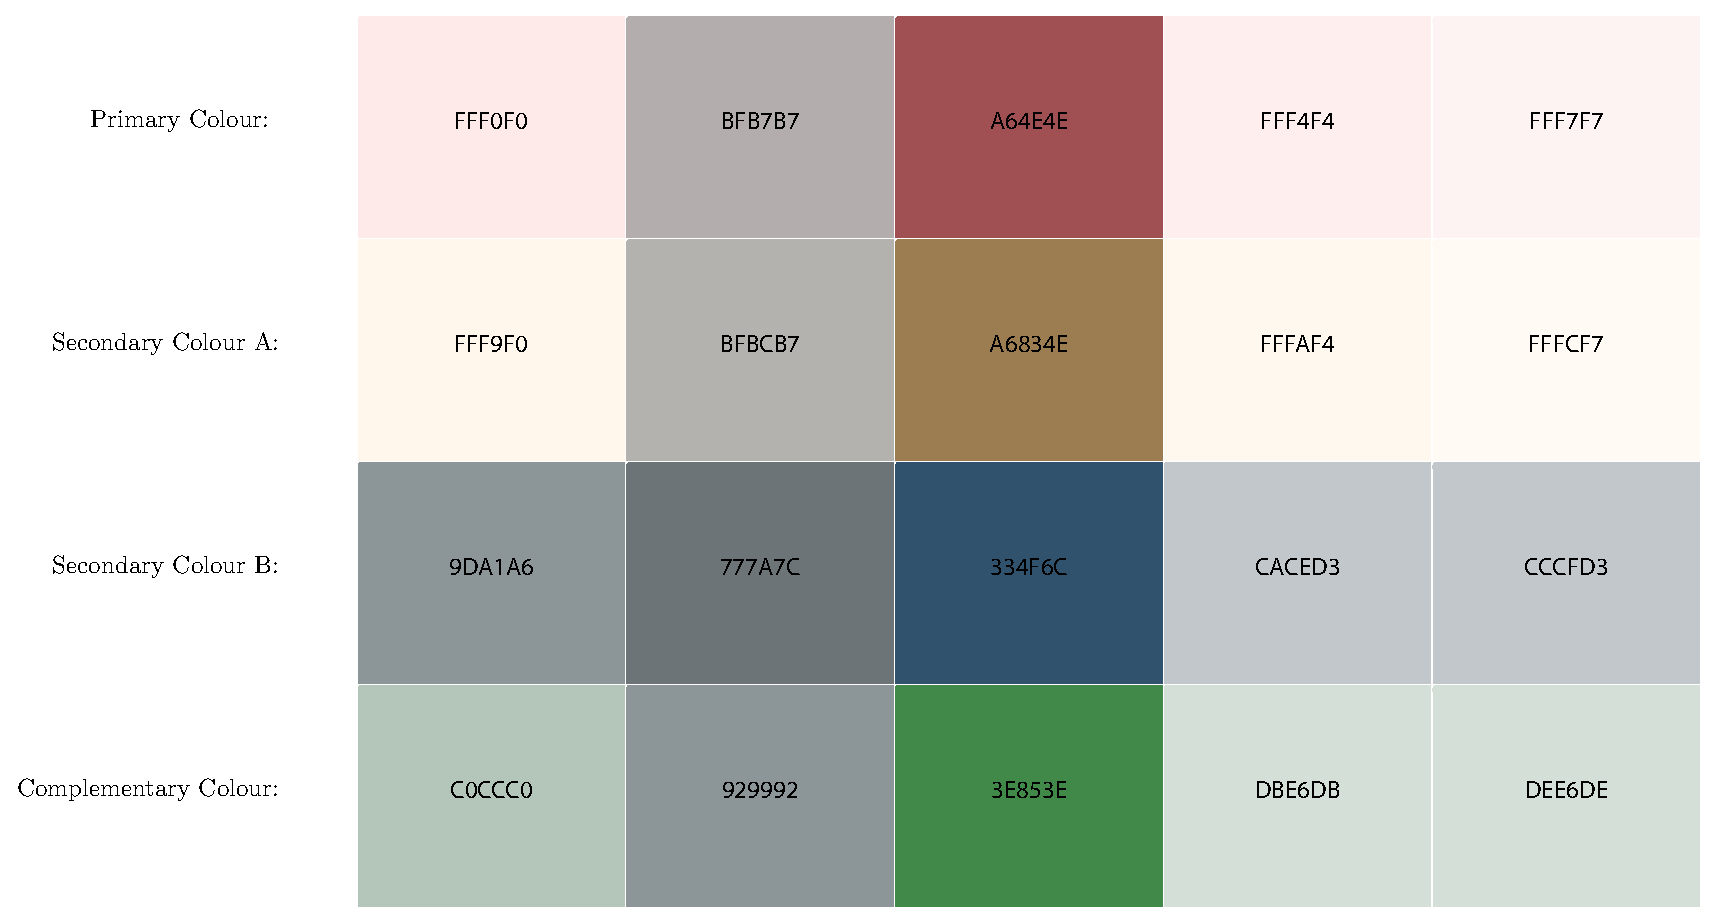
\includegraphics[width=.45\textwidth]{img/colour-scheme.eps}
	\caption{Colour scheme of the interface \protect\cite{colorschemedesigner.com}}
	\label{fig:colour-scheme}
\end{figure}
\todonote{colorschemedesigner.com cite}

\section{Test}




\section{Constraints}
The constraints can be divided into groups: layout-/content-based, global/topic/neighbouring, 


Technical argumentation for choices.
Business case argumentation for choices (user needs).
Reference to written articles about design choices - navigation: sections + headlines, 

\subsection{Layout Constraints}
first focus: layout + one sections

3? columns
images/no image
base layout



\subsection{Content Constraints}
Content similarity relationships:
article vs. neighbouring articles
article vs. containing section/topic
article vs. whole newspaper

``[...] it was found that the best eight-item  mix within an issue was not necessarily composed of the eight highest-readership items in that issue.'' \cite{EditorsDilemma} (maximum audience coverage, which is no longer an issue due to personalisation)

\begin{align*}
\mathcal{C} &=	\begin{Bmatrix}
					\texttt{all\_different}(a_i),\\
					\texttt{sim}(a_i, a_{i+1}, 0.7, 0.9), \\
					\texttt{sim}(a_i, a_{i-1}, 0.7, 0.9), \\
					\texttt{sim}(a_i, a_j, 0.3, 0.9)
					%artists_i \ne artists_{i-1} \wedge artists_i \ne artists_{i+1},\\
					%album_i \ne album_{i-1} \wedge album_i \ne album_{i+1},\\
					%\texttt{all\_different}(place_i),\\
					tempo_i < tempo_{i+1} + 10 \wedge tempo_i < tempo_{i-1} + 10 \wedge\\
					tempo_i > tempo_{i-1} - 10 \wedge tempo_i > tempo_{i+1} - 10,\\
					%tempo_i < + 5 \cdot length \cdot tempo_j \wedge\\
					%tempo_i > - 5 \cdot length \cdot tempo_j\ \textbf{for}\ i \ne j,\\
					%keys_i = keys_i \vee keys_i = keys_i \pm 1 \vee keys_i = keys_i \pm 12
				\end{Bmatrix}
\end{align*}


\todonote{AIRussel p. 207 preference constraints. can often be encoded as costs on individual variable assignments. Solved either path-based or local.
p. 216 Minimum-remaining-values, p. 217 Least-constraining-value.}

\section{Test Results}
long layout

Stumbleupon - Collaborate filtering for recommendation

% section analysis (end)

%!TEX root = thesis.tex
\chapter{Implementation} % (fold)
\label{ch:implementation}

\todonote{css: conditional styling}

\section{Server}

using hash of url as ids.

looking for images and videos in the article.

\subsection{Word tagging}
tagging: maxent\_treebank\_pos\_tagger, Treebank Part of Speech Tagger (Maximum entropy) - sikkert upenn corpus.
%upenn\_treebank.pdf

alternativt: Treebank Part of Speech Tagger (HHM)


wordnet\_enrich: ``W-kmeans: Clustering News Articles Using WordNet'', 116262780379.pdf

wordnet sammensatte ord

cite ``Text Classification Using WordNet Hypernyms.pdf''
hypen density. This is better in 116262780379.pdf

using nouns and adjectives NOT nouns and verbs as in ``Text Classification Using WordNet Hypernyms.pdf''


tagging på feeds er givet fra feedets navn. Kan bruges til at verificere min classification.



Opbygge en database med articler og bruge det som basis for similarity queries.
wordnet\_ic Information Content: Load an information content file from the wordnet\_ic corpus.
\begin{lstlisting}[caption=cap,label=lst:lab,float=htbp]
	>>> from nltk.corpus import wordnet_ic
	>>> brown_ic = wordnet_ic.ic('ic-brown.dat')
	>>> semcor_ic = wordnet_ic.ic('ic-semcor.dat')
	>>> dog.res_similarity(cat, brown_ic)
	7.9116665090365768
	>>> dog.res_similarity(cat, genesis_ic)
	7.1388833044805002
\end{lstlisting}



\section{Client Side}

worker.js to create a background worker to perform the constriant programming.

Model-View-Control using backbone.js

Paging: single page web apps + manipulation the browser history \url{https://developer.mozilla.org/en/DOM/Manipulating_the_browser_history}


Assignment from library in stead of arbitrary assignment? The latter is a more hypothetical approach. Providing the library as a constraint, where each variable assignment must have a unique combination from one of the possibilities of the constraint.
(sim,breaking,chars,date,sections?,columns):list


Ranges can be optimised in space by converting them to integer ranges. This can be done by setting min = 0 and max = (b-a)/gap.

Furthermore each subdomain should be able to be represented by a set of ranges and atomic values. Propagating through values causes many iterations and a whole range may be discarded by looking at its maximum and minimum value. However, if the range holds a potential valid value (solution to a variable) it can be divided into smaller ranges and their minimum and maximum values may be examined. This divide-and-conquer technique may continue until the search reaches atomic values (determined by the gap value of the range). If some atomic values and ranges seems to fulfil the constraints they should be returned. And the subdomain now consists of both ranges and atomic values.

Optimal/promising
fixed budget computation

The library could take any combination of constraints and then organise them into conjunctions of disjunctions, with the constraints taking fewer values first.

In the implementation this is done by hand, so the program takes conjunctions of disjunctions of constraints organised with constraints that takes fewer values first. Constraint weighing could also help organising the disjunctions and furthermore lead the search to concentrate on variables that is bound by these constraints. (p. 222 AIRussel).

Constraints should point to specific variables, this makes it somewhat rigid/ineffective because I have to write at global constraint that accounts for everything (ineffective in propagation -  might also be a problem if it does not show progress in changing values, i.e. it is a hard constraints and not returning a cost of the set of values.) or divide it into smaller constraints separated by an `or' (v). The latter is ineffective because there would should be a combination of constraints accounting for every situation, e.g. if the first variable is satisfying an unary constraint, the next say 3 variables (if the problem holds 4 variables) could satisfy three unary constraints, an unary and a binary (two combinations exists) or a constraint that takes three variables. This grows fast with the number of constraints.

\todonote{Does it make sense that a continuous range cannot have specific values removed? Should it be possible for it be divided into subranges if the user decides to remove a range of values in between its domain of [min;max]?}

% section design (end)
\include{09_discussion}
%!TEX root = thesis.tex
\chapter{Conclusion} % (fold)
\label{ch:conclusion}

% section conclusion (end)

% APPENDIX CHAPTERS INCLUDE
\appendix

% Appendix A, B, ...
%!TEX root = thesis.tex
%!TEX root = thesis.tex
\chapter{User Needs}
This section will define the user needs for the application.

\section{Personas}
%http://www.pewinternet.org/Reports/2010/Generations-2010.aspx 2010
%http://epp.eurostat.ec.europa.eu/portal/page/portal/statistics/search_database
%http://epp.eurostat.ec.europa.eu/tgm/table.do?tab=table&init=1&plugin=1&language=en&pcode=tin00097
%Individuals using the Internet for reading / downloading online newspapers / news magazines (tin00097)

\begin{itemize}
	\item \url{student} 35\%, \url{employees self-employed family workers} 31\%, unemployed, retired or other inactive
	\item \url{high formal education} 50\%, medium formal education, no or low formal education
	\item \url{male} 55\%, female
	\item \url{16-24} 34\%, \url{25-54} 34\%, 55-64, 65-74
\end{itemize}

\subsection{Thomas: student medium formal education male 21}
Thomas is 21 and a student at the Technical University of Denmark to be a bachelor of engineering in software. He is very interested in soccer and is therefore always updated on sports news. He reads about it online, newspapers and talks about it with friends. With big events he even likes to post it on Facebook. As a soon-to-be software engineer he has a natural thirst for news about technology, and he mainly reads these at home at the dormitory.
wired.com, newz.dk, engadget.com, facebook.com
computer, Samsung Galaxy Tab

\subsection{Laura: employed high formal education female 39}
Laura is 39 and is employed as a key account manager. She likes to be updated on strategies and economical status of rivalling companies. She is also very interested in politics and likes to discuss this subject with her friends. She reads economical news and likes to be updated on the run.
b.dk, borsen.dk, twitter.com
iPhone, iPad

\subsection{Marie: unemployed no or low formal education female 61}
Marie is 61 and a currently unemployed housekeeper. She spends her day looking for a job and taking care of her pet cat until her husband comes home. She mostly looks for the gossip sections or news about crime or big disasters. She also spends some time reading through the travelling guides as she dreams of going away with her husband.
ekstrabladet.dk, bt.dk, nyhederne.tv2.dk
computer, Lenovo IdeaPad A1

\subsection{Carl: retired or other inactive high formal education male 69}
Carl is a retired professor in psychology. He likes to discuss human behaviour and relation with his acquaintances and is very interested in cultural events. Therefore he often seeks the cultural sections and discussion fora to see what is going on. 
politiken.dk, aok.dk, dr.dk
computer, iPad

\section{Scenarios}
\subsection{Thomas}
Thomas comes home after a day at the study, picks up his tablet computer and opens Editor from the desktop. Editor opens and shows him the front page where all the headlines stories are displayed. The main story is about a new version of the Android OS that has been released today and presses it to read more. The story opens in a full window display with quality images to match the articles. He reads the first section and feels satisfied with the amount of information, but wants to share the information on Facebook, so he clicks share button and writes a comment and posts it on his Facebook wall. He closes the article and returns to the front page. He sees a top story below the main story about Mr. Mærsk Mc-Kinney Møller who has died. It is not a story that falls into his key interests, but as the news is big he is satisfied that he got informed about it. Thomas feels like reading more about technology so he opens the menu and chooses the ``Tech'' section he has installed in the application. The section opens with a head line and a page number to let him know where in his paper he has navigated to and finds an article about a new multicore CPU technology. He has never been interested in CPU technology before, but finds this technology interesting after reading about it, so he opens the application settings and types in keywords about the technology under his ``Tech'' section to keep him updated about it. He also adjusts the ratio between general and personal news, to be less personal as he feels like he needs to broaden his horizon a bit with respect to news. He closes the settings menu and Editor immediately starts updating the articles. Some new articles about CPU technology has been included amongst the articles in the ``Tech'' section after paging through the section and reading some of the most interesting articles he closes the application.

It could be nice if the key words of a story could be or is already highlighted, so he can click it and add it to his positive or negative list.

``Define keywords and user preferences as rules (static and ageing, dynamic)'' \cite{Personalizing-your-electronic-newspaper.pdf}

\subsection{Laura}
Laura is on the train on her way to a business meeting this morning and pulls out her tablet and sees she has one notification from Editor. She opens Editor to get updated on todays news. The front page is displayed and there are headlines from different top articles and a notification is shown in the corner. She presses the notification and the pages turns to show her the article, which opens in full screen. After reading it she wants to see todays headlines, so she presses the back button to return to the paper and presses the return to front page button and the paper turns pages to reach the front page. She scans the page to see if there is any big news about her rivalling companies. There is no breaking news, so she just turns the page to browse the content of todays paper. As she browses the ``Politics'' section of her paper she finds an article about the Prime Minister introducing a new bill about a toll ring around the capitol city. She chooses the article and it is shown in full screen. As she reaches the bottom of the article she sees the comments about it where her friends and most others are against it. She decides to join the discussion and posts a comment on the article wall. She also sees one of her friends has not commented on the article wall and decides to share the article with her as she thinks she would agree with her opinion. She presses the share button and chooses the Editor logo. A list of her friends is shown, some of them who has already read the article is greyed out, but the one she was looking for is not. So she chooses her and a notification is sent to her.

\subsection{Marie}
It is morning and Marie wants to check the news with her coffee in the couch, so she opens Editor from her tablet to get updated. The front page is displayed with a collection of stories as highlights of the content of the paper. It mainly contains stories about celebrities and a big disaster that has happened in japan, but there is also a story about a big political change, that she does not find interesting. So she goes to the settings menu and types in ``politics'' to add to her negative list. She also adjusts the personal/general news ratio to contain only personal news as she wants only news that is directed to her. She returns to the front page which is now free of political stories. Her newspaper contains many images and videos as she has set her graphical/textual content ratio more towards graphical content.

\subsection{Carl}
Cultural, funnies

\section{Business Case}

\subsection{Need}
User value: personal quality fresh stories (content providers should be chosen!) enriched with quality images. Same navigation as actual newspapers, but faster. Instantly up-to-date. Adaptive layout. Adjustable user profile.

\subsection{Approach}
personalised content + layout.

Constraint Programming: fast computation - good for optimal solutions, describes the generic solution in stead of how to solve or find it, very easy to tailor the problem definition of the solution and adjust it and even let users make the adjustments, transparent.

Content providers can get to know their readers preferences better and improve the provided content.

\subsection{Benefit Per Cost}
revenue flow: Content providers are paid. Income from advertisers (scattered \cite[p. 6-7]{kristin_fredrik.pdf}) and users. Income from selling user behaviour. Free version w. commercials + paid (monthly) without.

\subsection{Competition}
Flip board, Wired magazine and app with actual editors affiliated.

\todonote{Which design choices to focus on?}

\begin{itemize}
	\item ``open, turn pages, chose article, read and return'' \cite[p. 6]{FULLTEXT01.pdf}
	\item both general and personal news (collaborate filtering solves that some news are not received, but are universally interesting \cite{fulltext.pdf})
	\item full screen display of article
	\item images + video? adjustable
	\item graphical/textual content ratio
	\item opens in front page view (summery of newspaper 8 articles) \cite[p. 8]{kristin_fredrik.pdf}
	\item put in personalised sections
	\item back page, funnies?
	\item section headline \cite[p. 6-7]{kristin_fredrik.pdf}
	\item article headlines
	\item article summaries / extracts \cite{fulltext.pdf}
	\item menu w. section headlines \cite[p. 8]{kristin_fredrik.pdf}
	\item page numbers \cite[p. 6-7]{kristin_fredrik.pdf}
	\item page turn
	\item press ``like'' or key word based user profile (mark self or highlighted? right click to add): positive + negative list (keywords+categories \cite{10-1-1-19-5583}, \cite{fulltext.pdf} and \cite{gervasum2001ws.pdf})
	\item adjust variables
	\item share social network
	\item share directly (grey out the ones who have read it)
	\item comment
	\item see friends comments
\end{itemize}

\section{Technical Requirements}
\begin{itemize}
	\item ``the clear overview of content, including a beginning and an end, the ease of use, typography and design'' \cite[p. 7]{FULLTEXT01.pdf}
	\item familiarity in design from printed paper \cite[p. 7]{FULLTEXT01.pdf}
	\item  ``news valuation, e.g. positioning of lead story'' \cite[p. 7]{FULLTEXT01.pdf}
	\item  mobility \cite[p. 7]{FULLTEXT01.pdf}
	\item  continuous updates \cite[p. 7]{FULLTEXT01.pdf}
	\item  ability to search \cite[p. 7]{FULLTEXT01.pdf}
	\item  ``easy and intuitive navigation'' \cite[p. 7]{FULLTEXT01.pdf}
	\item add video and sound \cite[p. 7]{FULLTEXT01.pdf}
	\item Landscape + portrait \cite[p. 6-7]{kristin_fredrik.pdf}
	\item touch screen interaction \cite[p. 6-7]{kristin_fredrik.pdf}
	\item Design+layout from printed newspaper \cite{hcii2005_1004.pdf}
	\item Functionality from online newspaper \cite{hcii2005_1004.pdf}
	\item Name of columnist \cite[p. 4]{gervasum2001ws.pdf}
	\item Transparency of implicit relevance feedback (see/modify current weights of categories) \cite[p. 7]{gervasum2001ws.pdf}
	\item dynamic short-term + static long-term user profile \cite{10-1-1-19-5583}, \cite{fulltext.pdf} and \cite{gervasum2001ws.pdf}
	\item relevance feedback \cite{10-1-1-19-5583}, \cite{fulltext.pdf} and \cite{gervasum2001ws.pdf}
\end{itemize}

In which period of time is an article relevant to a user? Maybe if it is still available, then it is still interesting - new approaches or discussion about the subject might arise. How do we control that a news item is not missed? Keep index of what has been viewed in addition to what has been read.

\backmatter

\chaptermark{Bibliography}
\renewcommand{\sectionmark}[1]{\markright{#1}}
\sectionmark{Bibliography}

%%%%%%%BIBLIOGRAPHY INCLUDE%%%%%%%%%%%%%%%%%%%%%%%%%%%%%%%%%%%%%%%%%%%%%%

\bibliography{thesis}    % Bibliography
\bibliographystyle{lib/named}

\end{document}